%%%%%%%%%%%%%%%%%%%%%%%%%%%%%%%%%%%%%%%%%%%%%%%%%%%%%%%%%%%%%%%%%%%%%%%%%%%%%%%%%%%%
% Document data
%%%%%%%%%%%%%%%%%%%%%%%%%%%%%%%%%%%%%%%%%%%%%%%%%%%%%%%%%%%%%%%%%%%%%%%%%%%%%%%%%%%%
\documentclass[12pt]{report} %report allows for chapters
\renewcommand\thesection{\arabic{section}} % ignore the title number for sections
%%%%%%%%%%%%%%%%%%%%%%%%%%%%%%%%%%%%%%%%%%%%%%%%%%%%%%%%%%%%%%%%%%%%%%%%%%%%%%%%%%%%




%%%%%%%%%%%%%%%%%%%%%%%%%%%%%%%%%%%%%%%%%%%%%%%%%%%%%%%%%%%%%%%%%%%%%%%%%%%%%%%%%%%%
% Packages
%%%%%%%%%%%%%%%%%%%%%%%%%%%%%%%%%%%%%%%%%%%%%%%%%%%%%%%%%%%%%%%%%%%%%%%%%%%%%%%%%%%%
\usepackage{color, soul, xcolor} % Colored text and highlighting, respectively

%Tikz
\usepackage{tikz-cd} % For commutative diagrams
\usepackage{tikz-3dplot}
\RequirePackage{pgfplots}
\usetikzlibrary{shadows}
\usetikzlibrary{shapes}
\usetikzlibrary{decorations}
\usetikzlibrary{arrows,decorations.markings} 
\usetikzlibrary{quotes,angles}

\usepackage{mathtools}
\usepackage{answers}
\usepackage{setspace}
\usepackage{graphicx}
\usepackage{enumerate}
\usepackage{multicol}
\usepackage{mathrsfs}
\usepackage[margin=1in]{geometry} 
\usepackage{amsmath,amsthm,amssymb}
\usepackage{marvosym,wasysym} %fucking smileys
\usepackage{float}
\usepackage{morefloats}
%%%%%%%%%%%%%%%%%%%%%%%%%%%%%%%%%%%%%%%%%%%%%%%%%%%%%%%%%%%%%%%%%%%%%%%%%%%%%%%%%%%%




%%%%%%%%%%%%%%%%%%%%%%%%%%%%%%%%%%%%%%%%%%%%%%%%%%%%%%%%%%%%%%%%%%%%%%%%%%%%%%%%%%%%
% Shortcuts
%%%%%%%%%%%%%%%%%%%%%%%%%%%%%%%%%%%%%%%%%%%%%%%%%%%%%%%%%%%%%%%%%%%%%%%%%%%%%%%%%%%%
% Number systems
\newcommand{\N}{\mathbb{N}}
\newcommand{\Z}{\mathbb{Z}}
\newcommand{\C}{\mathbb{C}}
\newcommand{\R}{\mathbb{R}}
\newcommand{\Q}{\mathbb{Q}}

% Operators/functions
\newcommand{\id}{\mathrm{Id}}
\DeclareMathOperator{\sech}{sech}
\DeclareMathOperator{\csch}{csch}
%%%%%%%%%%%%%%%%%%%%%%%%%%%%%%%%%%%%%%%%%%%%%%%%%%%%%%%%%%%%%%%%%%%%%%%%%%%%%%%%%%%%




%%%%%%%%%%%%%%%%%%%%%%%%%%%%%%%%%%%%%%%%%%%%%%%%%%%%%%%%%%%%%%%%%%%%%%%%%%%%%%%%%%%%
% Environments
%%%%%%%%%%%%%%%%%%%%%%%%%%%%%%%%%%%%%%%%%%%%%%%%%%%%%%%%%%%%%%%%%%%%%%%%%%%%%%%%%%%%
% Italic font
\newtheorem{theorem}{Theorem}[section]
\newtheorem{lemma}{Lemma}[section]
\newtheorem{corollary}{Corollary}[section]
\newtheorem{axiom}{Axiom}

% Plain font
\theoremstyle{definition}
\newtheorem{definition}{Definition}[section]
\newtheorem{example}{Example}[section]
\newtheorem{remark}{Remark}[section]
\newtheorem{solution}{Solution}
\newtheorem{problem}{Problem}[section]
\newtheorem{question}{Question}[section]
\newtheorem{answer}{Answer}[section]
\newtheorem{exercise}{Exercise}[section]
%%%%%%%%%%%%%%%%%%%%%%%%%%%%%%%%%%%%%%%%%%%%%%%%%%%%%%%%%%%%%%%%%%%%%%%%%%%%%%%%%%%%

\begin{document}


\begin{center}
   \textsc{\large MATH 255, Homework 10: \emph{Solutions}}\\
\end{center}
\vspace{.5cm}

\noindent\textbf{Problem 1.} Imagine a stream of water on the surface of a river that carries a particle along. The stream velocity is given by
\[
\mathbf{v}(x,y)=\begin{bmatrix} v_1 \\ v_2 \end{bmatrix},
\]
with $v_1$ and $v_2$ constant. We want to find the trajectory of the particle that begins at the point $(x_0,y_0)$ at time $t=0$.
\begin{enumerate}[(a)]
    \item Let $\mathbf{x}(t)$ give the position of the particle at time $t$. Write the differential equation that satisfies the following statement:
    
    \emph{At each time $t$, the particle's velocity is equal to the velocity of the stream at that point.}
    
    \item Find the particular solution $\mathbf{x}(t)$ that satisfies our initial condition $\mathbf{x}(0)=(x_0,y_0)$.
    
    \item Now let $(v_1,v_2)=(5,2)$ and $(x_0,y_0)=(1,2)$.  What is the particular solution? 
\end{enumerate}
The advantage to solving problems in this way (i.e., solving as we do in (b) and then using this to solve (c)) is that we have solved a problem that can be changed to suit another future problem.  Leaving parameters in problems is highly advantageous.
\begin{solution}~
\begin{enumerate}[(a)]
    \item The differential equation described here is to take the particle's velocity $\mathbf{x}'(t)$ (the derivative of the position $\mathbf{x}(t)$) and set it equal to the stream velocity $\mathbf{v}$.  So we have
    \[
    \mathbf{x}'=\mathbf{v}.
    \]
    Specifically, we have
    \[
    \begin{bmatrix} x'(t) \\ y'(t) \end{bmatrix} = \begin{bmatrix} v_1 \\ v_2 \end{bmatrix}.
    \]
    \item We have two uncoupled equations
    \begin{align*}
        x' &= v_1,\\
        y' &= v_2,
    \end{align*}
    which can both be integrated to find
    \begin{align*}
        x(t) &= v_1 t +c_1,\\
        y(t) &= v_2 t +c_2.
    \end{align*}
    Noting that we want
    \[
    \mathbf{x}(0)=\begin{bmatrix} x_0 \\ y_0 \end{bmatrix}
    \]
    we get
    \[
    x(0)=x_0=v_1(0)+c_1
    \]
    which means $c_1=x_0$. Similarly,
    \[
    y(0)=y_0=v_2(0)+c_2
    \]
    which means $c_2=y_0$.  So our particular solution is
    \[
    \mathbf{x}(t) = \begin{bmatrix} v_1t+x_0 \\ v_2t+y_0 \end{bmatrix}.
    \]
    \item We simply plug in these values and find
    \[
    \mathbf{x}(t) = \begin{bmatrix} 5t+1 \\ 2t+2 \end{bmatrix}.
    \]
\end{enumerate}
\end{solution}

\begin{center}\underline{Problems 2-4 are all related.}
\end{center}

\noindent\textbf{Problem 2.} Consider the nonlinear second order ODE 
\[
x''- (1-x^2)x'+x = 0.
\]
This is known as the \emph{Van der Pol oscillator}. It models a certain type of mass/spring system. In this case, I have set a parameter $\mu=1$ for simplicity.
\begin{enumerate}[(a)]
    \item Why is this equation nonlinear?
    \item Letting $y=x'$, rewrite this equation as a system of two first order ODE. That is, one equation for $x'$ and the other for $y'$. \emph{Note that $x'$ is a velocity.}
    \item Plot the vector field given by this system. \emph{Note that this vector field lives in \underline{phase space}. That is, one axis is position and the other is velocity.}
    \item Using the vector field plot and the ODE itself, predict how this system evolves over time. 
\end{enumerate}
\begin{solution}~
\begin{enumerate}[(a)]
    \item This equation is nonlinear since it cannot be written as
    \[
    x''+f(t)x'+g(t)x=h(t).
    \]
    Specifically, there is the term 
    \[
    (1-x^2)x'
    \]
    that prevents this equation from being linear.
    \item We let $y=x'$ which means that we have $y'=x''$.  If we substitute these into our ODE, we have
    \[
    y'-(1-x^2)y+x=0
    \]
    is first order in $y$.  Thus, our system of ODE is
    \begin{align}
        x'&=y,\\
        y'&=(1-x^2)y-x.
    \end{align}
    \item The vector field we plot is given by the system we found. Specifically, plot
    \[
    \mathbf{x}' = \begin{bmatrix} y\\ (1-x^2)y-x) \end{bmatrix}.
    \]
    This plot looks like
    \begin{figure}[H]
        \centering
        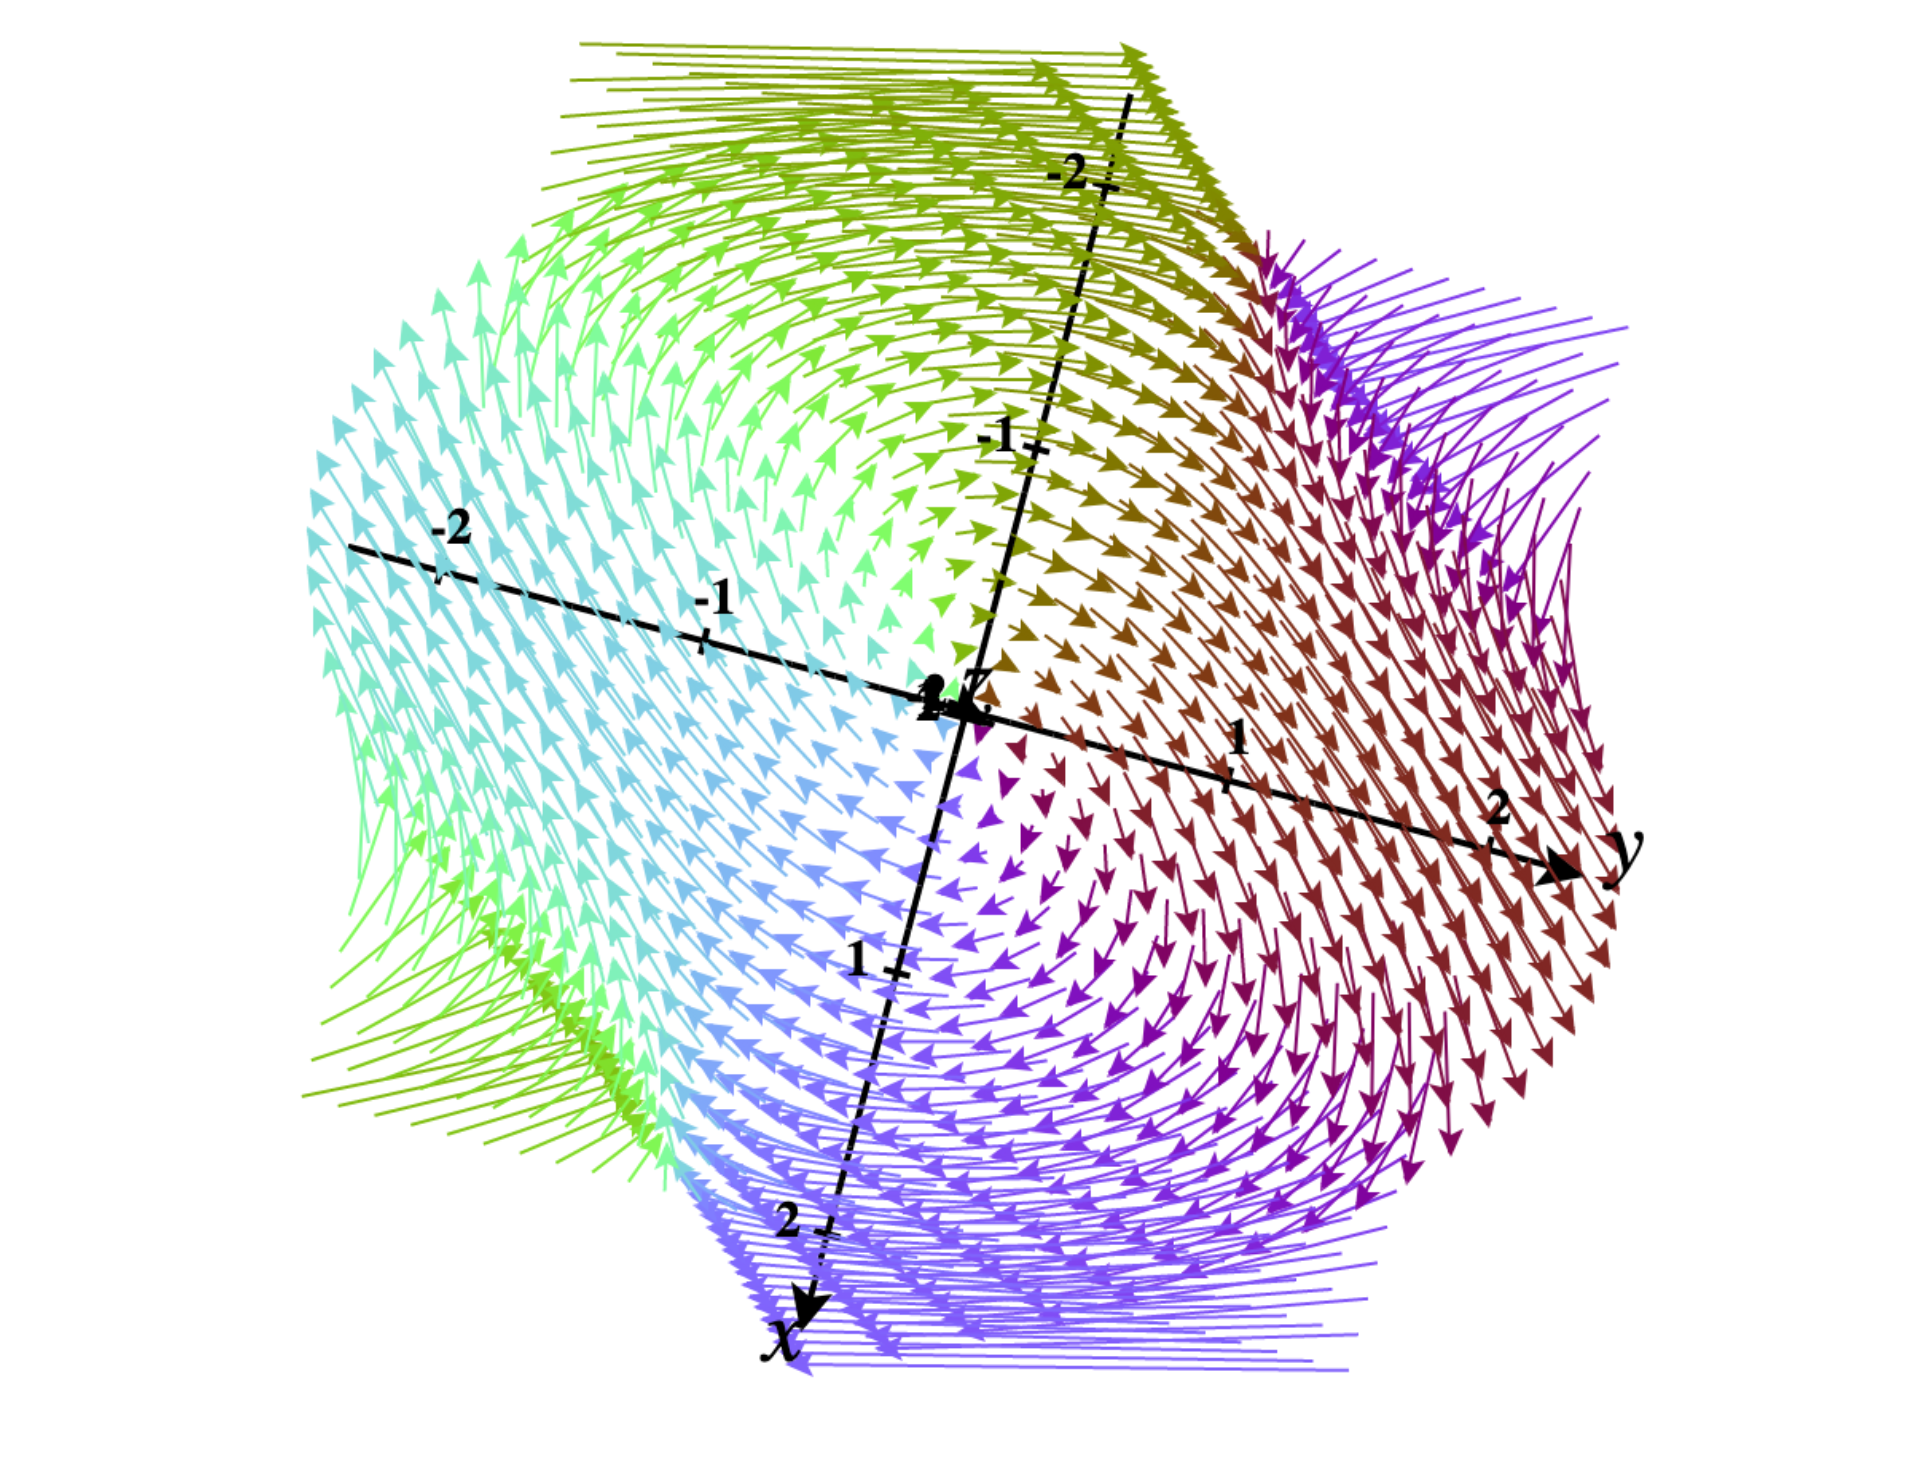
\includegraphics[width=.5\textwidth]{Images/vanderpol.png}
        \caption{Vector field for the Van der Pol oscillator.}
    \end{figure}
    \item The differential equation is similar to the Harmonic oscillator, but with an extra $x'$ term.  Based on this, and the vector field, it seems like there is due to be oscillatory behavior for this system.  Whether or not trajectories grow or shrink in magnitude is not immediately obvious.
\end{enumerate}
\end{solution}
\vspace*{.5cm}

\noindent\textbf{Problem 3.} Now that we have rewritten the second order equation as system of first order ODE, we now want to solve this problem.  To solve this, we need to linearize.
\begin{enumerate}[(a)]
    \item Taking your planar system from Problem 2, linearize the system about the point $(0,0)$. 
    \item Taking same nonlinear system, linearize instead about the point $(1,1)$.  
    \item What are differences in the matrices you got for (a) and (b)? 
\end{enumerate}
\begin{solution}~
\begin{enumerate}[(a)]
    \item From 2 we have,
    \begin{align*}
        x'&=y,\\
        y'&=(1-x^2)y-x.
    \end{align*}
    We must compute the partial derivatives
    \begin{align*}
        \frac{\partial x'}{\partial x} &= 0, & \frac{\partial x'}{\partial y}&=1,\\
        \frac{\partial y'}{\partial x} &= -2xy-1, & \frac{\partial y'}{\partial y}&=1-x^2.
    \end{align*}
    Evaluating these partials at the point $(0,0)$ gives us the linearization matrix
    \[
    M_{(0,0)}= \begin{bmatrix} 0 & 1\\ -1 & 1\end{bmatrix}.
    \]
    \item Instead, at the point $(1,1)$, we evaluate these partials and get the linearization matrix
    \[
    M_{(1,1)}=\begin{bmatrix} 0 & 1 \\ -3 & 0 \end{bmatrix}.
    \]
    \item The matrix $M_{(1,1)}$ has one more zero than the matrix $M_{(0,0)}$.  This will affect the dynamics quite a bit.
\end{enumerate}
\end{solution}
\vspace*{.5cm}

\noindent\textbf{Problem 4.} Let's concentrate on solving the linear problem about each of the above points. Your linearizations around $(0,0)$ and $(1,1)$ takes the form
    \[
    \mathbf{v}'=M\mathbf{v},
    \]
    where $M$ is a $2\times2$-matrix and 
    \[
    \mathbf{v}= \begin{bmatrix} x \\ y \end{bmatrix}.
    \]
\begin{enumerate}[(a)]
    \item Find the eigenvalues of the matrix found by linearizing around $(0,0)$.
    \item Find the eigenvalues of the matrix found by linearizing around $(1,1)$.
    \item What is the general solution for the linear system about $(0,0)$?
    \item What is the general solution for the linear system about $(1,1)$?
    \item How do these different linearizations behave? Are they the same? If not, what is different?
\end{enumerate}
\begin{solution}~
\begin{enumerate}[(a)]
    \item The eigenvalues of the matrix $M_{(0,0)}$ are
    \begin{align*}
    \lambda_1 &= \frac{1}{2}(1+i\sqrt{3}), & \lambda_2&= \frac{1}{2}(1-i\sqrt{3}).
    \end{align*}
    \item The eigenvalues of the matrix $M_{(1,1)}$ are
    \begin{align*}
    \lambda_1 &= i\sqrt{3}, & \lambda_2&= -i\sqrt{3}.
    \end{align*}
    \item The general solution about $(0,0)$ is then
    \[
    x(t)=Ae^{t/2} \sin\left( \frac{\sqrt{3}}{2}t\right) + Be^{t/2}\cos \left(\frac{\sqrt{3}}{2}t \right).
    \]
    \item The general solution about $(1,1)$ is then
    \[
    x(t)= A \sin(\sqrt{3}t) + B \cos (\sqrt{3}t).
    \]
\end{enumerate}
\end{solution}
\vspace*{.5cm}

\noindent\textbf{Problem 5.} One other common type of ordinary differential equation are the \emph{exact} equations.  They are very much related to potential fields that we have previously discussed. This form shows up more often in thermodynamics just due to the nature of the problems.

Let our differential equation be
\[
x' = \frac{-x-1}{t+1}.
\]
\begin{enumerate}[(a)]
\item Rewrite this equation in the form
\[
P(x,t)dx + Q(x,t)dt = 0.
\]
\item Show this equation is exact by showing
\[
\frac{\partial P}{\partial t} -  \frac{\partial Q}{\partial x} = 0.
\]
\item Since this equation is exact, we can integrate $P(x,t)$ with respect to $x$ determine the solution function up to some additional function of just $t$, $f(t)$.

\item Repeat this, but integrate $Q(x,t)$ with respect to $t$ to determine the solution function up to up some additional function of just $x$, $g(x)$.
\item This you should now have determined an $F(x,t)$ that is correct up to some constant.  Set this $F(x,t)$ (with the constant) equal to $0$ and solve for $x$ to find $x(t)$.  This is your solution.
\end{enumerate}
\begin{solution}~
\begin{enumerate}[(a)]
    \item We begin with 
    \[
    x' = \frac{dx}{dt}=\frac{-x-1}{t+1}.
    \]
    So we put it in the form as shown.
    \begin{align*}
        \frac{dx}{dt}&=\frac{-x-1}{t+1}\\
        dx &= \frac{-x-1}{t+1}dt\\
        (t+1)dx &= (-x-1)dt\\
        (t+1)dx+(-x-1)dt &=0.
    \end{align*}
    So, $P(x,t)=t+1$ and $Q(x,t)=x+1$.  
    \item We compute
    \[
    \frac{\partial P}{\partial t} = 1, \quad \textrm{and} \quad \frac{\partial Q}{\partial x} = 1.
    \]
    Thus it follows that
    \[
    \frac{\partial P}{\partial t}-\frac{\partial Q}{\partial x}=1-1=0.
    \]
    \item We integrate 
    \[
    \int P(x,t)dx = \int t+1 dx = xt+x + f(t).
    \]
    \item Again, integrate
    \[
    \int Q(x,t)dt = \int x+1 dt = xt + t + g(x).
    \]
    \item So, both the above functions must be equal. In fact, we have
    \[
    F(x,t) = xt+x+f(t)= xt+t+g(x).
    \]
    Now, we can see that
    \begin{align*}
        xt+x+f(t)&=xt+t+g(x)\\
        x+f(t)&=t+g(x)\\
        f(t)-g(x)&= t-x.
    \end{align*}
    So we can see that $f(t)=t$ and $g(x)=x$ from here.  However, we really have only determined $F(x,t)$ up to some constant $c$, thus
    \[
    F(x,t) = xt+x+t+c.
    \]
    Now, we set $F(x,t)=0$ to find our solution. So we have
    \begin{align*}
        F(x,t) &= 0\\
        xt+x+t+c&=0\\
        xt+x&=-t-c\\
        x(t+1)&=-t-c\\
        x=\frac{-t-c}{t+1}.
    \end{align*}
\end{enumerate}

\end{solution}




\end{document}  